\begin{center}
    \chapter{Cadre général du projet}
\end{center}

%Intro\footnotemark\\
%note en bas de page

\textbf{\huge Introduction} \\[1cm]



%inclusion d'une mage dans le document
%\begin{figure}[!h]
%\begin{center}
%taille de l'image en largeur
%remplacer "width" par "height" pour régler la hauteur
%\fbox{\includegraphics[width=15cm]{presentation/schema}
%\end{center}
%légende de l'image
%\caption{Schéma descriptif}
%\end{figure}

%Contenu de la note précédemment marquée avec \footnotemark
%\footnotetext{Note bas de page "intro"}
\textsf{\LARGE 
Ce chapitre est consacré à la présentation du cadre général de notre projet. En premier lieu, nous présentons la société d’accueil. Par la suite, nous présentons le cadre du projet qui comporte la problématique. On finit par une présentation de la méthodologie que nous allons adopter pour le développement de notre projet.}\\[1cm]

%retour à la ligne (alinea)

%saut de paragraphe

%\newpage

\section{Société d’accueil  }
\textsf{\LARGE 
Dans ce qui suit,nous présentons la société d'accueil ainsi que son domaine d'activié.\\[1cm]
\subsection{   Identité }
\texttt{}\\[0.5cm]
\textsf{\LARGE Mobelite est une agence spécialisée dans le conseil en stratégie mobile, la conception et le développement d’applications mobiles et de sites web et le marketing mobile. Mobelite est forte d’une équipe d’experts dans la réalisation d’applications mobiles sur les plateformes les plus répandues et les applications Web. Mobelite dispose d’équipes commerciales et marketing à Paris (France), et d’équipes de développement à Tunis et Monastir (Tunisie).
}
\begin{figure}
\begin{center}
%taille de l'image en largeur
%remplacer "width" par "height" pour régler la hauteur
\fbox{
\includegraphics[width=10cm]{presentation/opg}}

\end{center}
%légende de l'image
\caption{Logo de la société mobelite}
\end{figure}
\newpage
\subsection{ Activités de mobelite}
\texttt{}\\[0.5cm]
\textsf{\LARGE Mobelite experts dans la création des sites web intuitifs et ergonomiques pour tous les supports soit desktop, tablette ou mobile et avec les plus récents technologies et Framework de développement comme React JS, Node JS et Angular. Mobelite aussi maîtrisons parfaitement la conception et le développement d’applications natives iOS et Android pour tous les diffèrent supports smartphone, tablette, Watch et TV. Mobelite excelle dans le guidage de ses clients dans différentes parties de projets comme l'analyse des besoins, UX/UI, conception, design, développement, SEO, DevOps, hébergement. Tout ça est réalisés selon la méthodologie Agile, afin de maximiser les possibilités d’itérations sur le concept, et d’introduire plus de flexibilité sur les arbitrages fonctionnels à faire.
}
\begin{figure}
\centering
\fbox{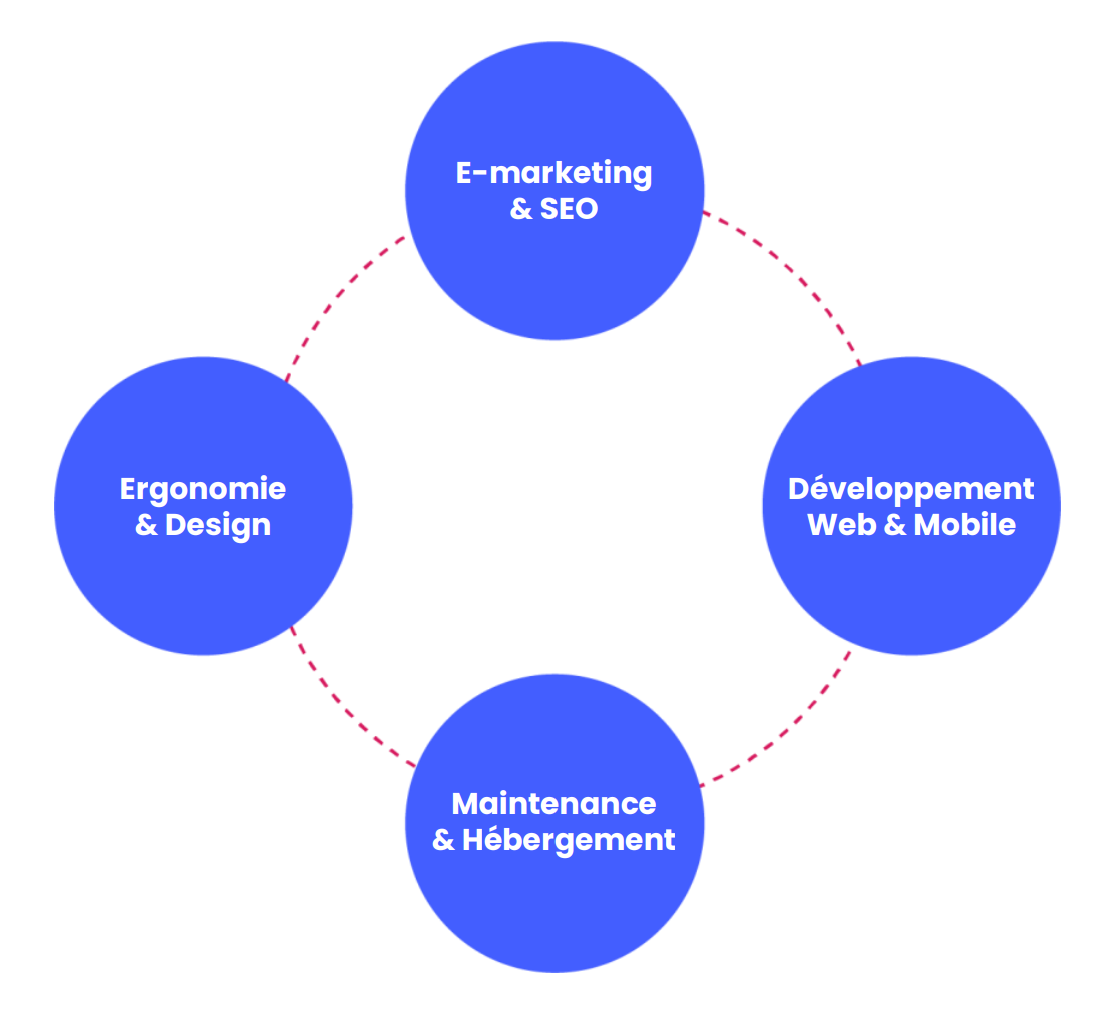
\includegraphics[width=10cm]{presentation/domaine.png}}
\caption{différents domaines de mobelite}
\label {fig:Activités de mobilite}
\end{figure}
\newpage
\section{Problématique }
\texttt{}\\[0.5cm]
\textsf{\LARGE
Le déploiement des systèmes de gestion de code source tell que Nexus, SonarQube  sur un seul serveur local présent plusieurs problèmes qui affecte la performance de serveur et qui rend l’exécution des diffèrent application ou l’ajout des nouvelles fonctionnalités plus difficile aussi la maintenance de plusieurs applications au même temps sera compliquée et nécessite une planification minutieuse pour éviter l’interruption des processus d’autres applications, les besoins d’entreprise changer au cours des temps et la capacité d'un seul serveur sera insuffisante pour rependre à la charge des données, les mise à jour des applications peut impact autre application ou seront impossibles à cause de limites des ressources, on terme de sécurité une attaque sur le serveur cause un perd des données très grand que sera difficile de restaurer en conséquence de l’utilisation d'un seul serveur.
}
\section{Méthodologie de développement}
\texttt{}\\[0.5cm]
\textsf{\LARGE Pour la réalisation de notre projet nous avons opté pour la méthodologie agile SCRUM car elle améliorer la flexibilité de projet et réduit le temps de livraison de produits complet au client.
}
\subsection{\Large  Présentation de la méthode Scrum}
\texttt{}\\[0.5cm]
\textsf{\LARGE Scrum est une méthodologie agile pour l'élaboration, la réalisation et le soutien de projets complexes. Elle est basée sur la division du produit sur différentes itérations nommé sprints. Scrum est plus utile lorsque les exigences sont variables et qu’il peut changer beaucoup au cours du cycle de vie, elle donne donc la Capacité d'avoir un projet flexible capable de traiter les changements fréquents.
}
\subsection{\Large    Acteur de la méthode Scrum}
\texttt{}\\[0.5cm]

\par \noindent \textbf{\Large Scrum Master}:\textsf{\LARGE Il s'agit de la personne chargée d'orienter l'équipe de travail vers la bonne voie, d'assurer la bonne pratique des règles de la méthode Scrum et d'organiser son équipe.} \\[0.1cm]

\noindent \textbf{\Large Product Owner}: \textsf{\LARGE il représente les clients et assure que leurs besoins et visions soient réalisés dans le projet, il travaille généralement en collaboration directe avec l’équipe de développement. }\\[0.1cm]

\noindent \textbf{\Large Equipe de développement}:\textsf{\LARGE sont les personnes responsables de la transformation des besoins du client qu'ils sont définis par le Product Owner a des fonctions utilisables, l'équipe est composée d'au moins 3 personnes jouant les rôles de développeur ou de concepteur.}\\[0.1cm]
\subsection{\Large Évènements de la méthode Scrum }
 \texttt{}\\[0.1cm]
\textsf{ \LARGE Scrum définit cinq évènements : }
\\[0.1cm]

\par \noindent \textbf{\Large - Le sprint  }:\textsf{\LARGE chaque sprint est de durée maximale de 4 semaines pendant laquelle une version de produit est réalisée, à la fois un sprint termine un nouveau commencé avec une liste de fonctionnalités et un objectif à réaliser.} \\[0.1cm]

\noindent \textbf{\Large - Planification d’un sprint }: \textsf{\LARGE À chaque début de sprint cette réunion est conçue pour déterminer les tâches à réaliser pendant le sprint, l’organisation de ses tâches effectuées par l’équipe de développement et le Product Owner. }\\[0.1cm]

\noindent \textbf{\Large - Mêlée quotidienne }:\textsf{\LARGE est une réunion de durée 15 minutes font par l’équipe chaque jour pour définir l’objectif de journée et identifier les obstacles s’il y en a quelques-uns.}\\[0.1cm]
\noindent \textbf{\Large - Revue de sprint  }:\textsf{\LARGE Représente le travail réalisé par l’équipe au cours du sprint et le comparer avec le produit imaginé.}\\[0.1cm]
\noindent \textbf{\Large - Rétrospective de sprint   }:\textsf{\LARGE le but de cet événement est détermine les problèmes intervenus dans la période de sprint, l’efficacité des outils et déterminés ce qui peut être amélioré.}\\[0.1cm]

\subsection{ \Large Les artefacts}
\texttt{}\\[0.5cm]
\noindent \textbf{\Large - Product Backlog   }:\textsf{\LARGE il s’agit d’une liste des besoins et exigences recueillent pour créer le produit désiré, ce document est la responsabilité de Product Owner.}\\[0.1cm]
\noindent \textbf{\Large -  Sprint Backlog   }:\textsf{\LARGE c’est l’ensemble des données permet la réalisation d’objectifs de sprint, ce document est mis à jour par l’équipe de développement régulièrement.}
\texttt{}
\newpage
\begin{figure}
\begin{center}
%taille de l'image en largeur
%remplacer "width" par "height" pour régler la hauteur
\fbox{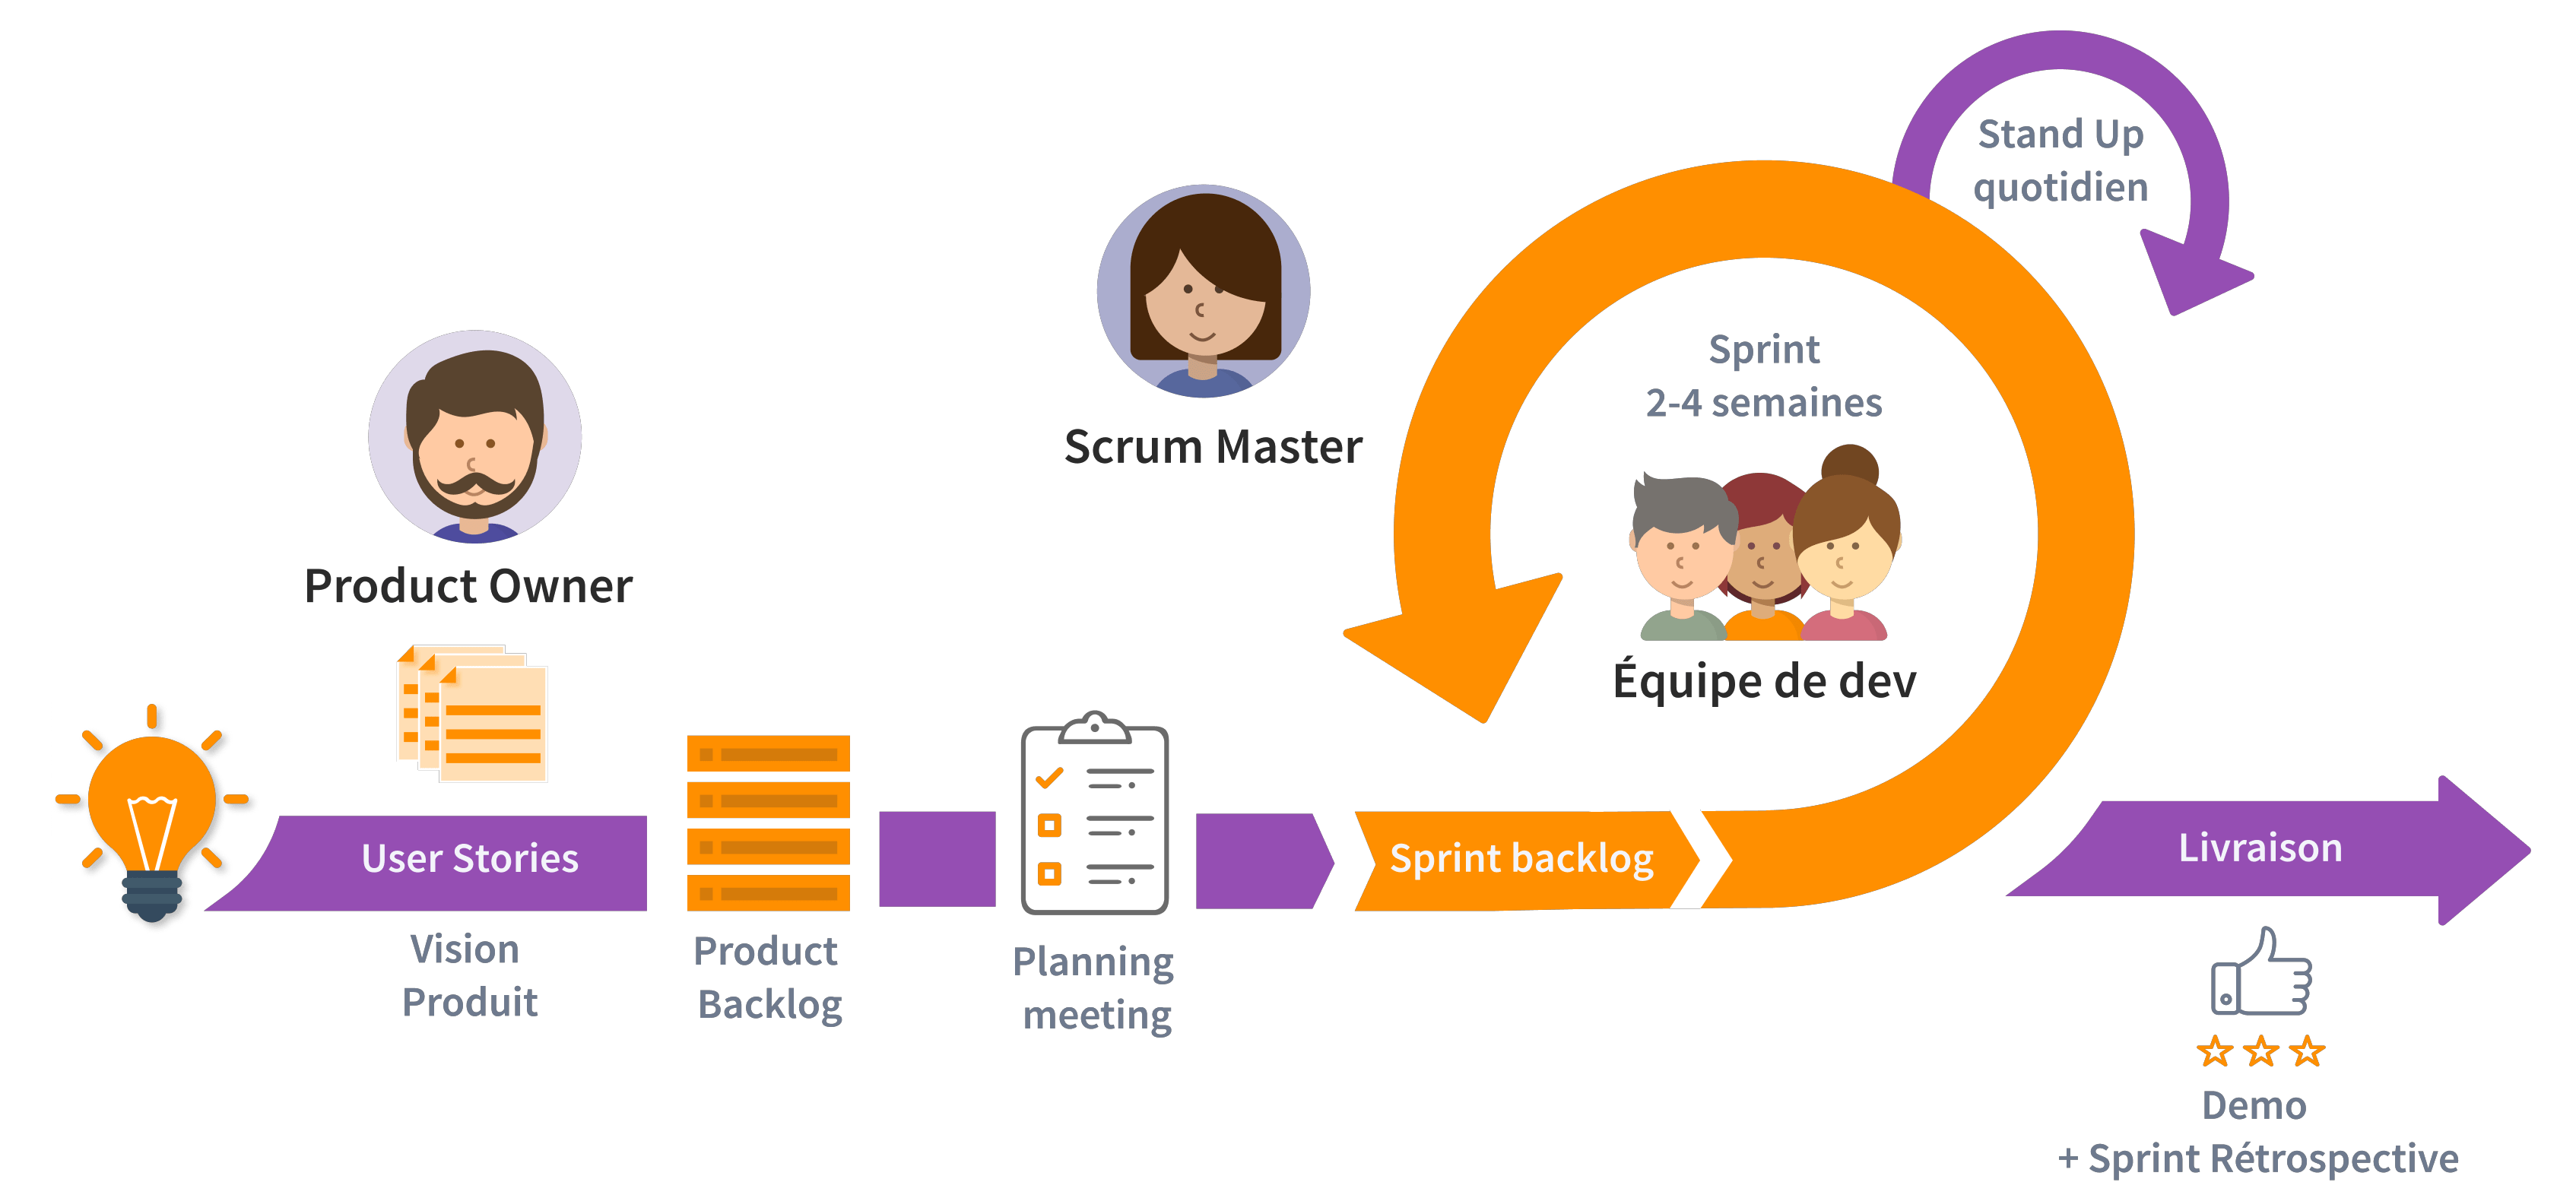
\includegraphics[height=7cm]{agile-Scrum-sprint-workflow-schema-FR.png}}
\end{center}
%légende de l'image
\caption{processus de méthode Scrum}
\end{figure}
\section{\LARGE    conclusion}
\texttt{}\\[0.3cm]
\textsf{\LARGE Dans ce chapitre nous avons présenté la société d’accueil et nous avons invoque la problématique et la méthodologie de développement.
Dans le prochain chapitre, nous allons faire une étude d’existant et faire une comparaison puis présenté la solution proposée.
}
%Voici une liste :
%\begin{itemize}
%\item item 1;
%\item item 2;
%\item item 3;
%\item item 4.
%\end{itemize}

%Comment :
%\footnotemark\\

%Detail :
%citation référencé dans le document "bibliographie.bib" inclus à la fin du document

%\footnotetext